% Subsampling: Kopien des Bandpass-Spektrums. Farbe = Verschiebung k*f_s (Tick auf der Achse = gleiche Farbe wie die zwei Rechtecke).
% Oben f_s im Fenster, unten ausserhalb. Einheiten beliebig: f_l=3, f_u=5.
\begin{center}
\resizebox{.92\linewidth}{!}{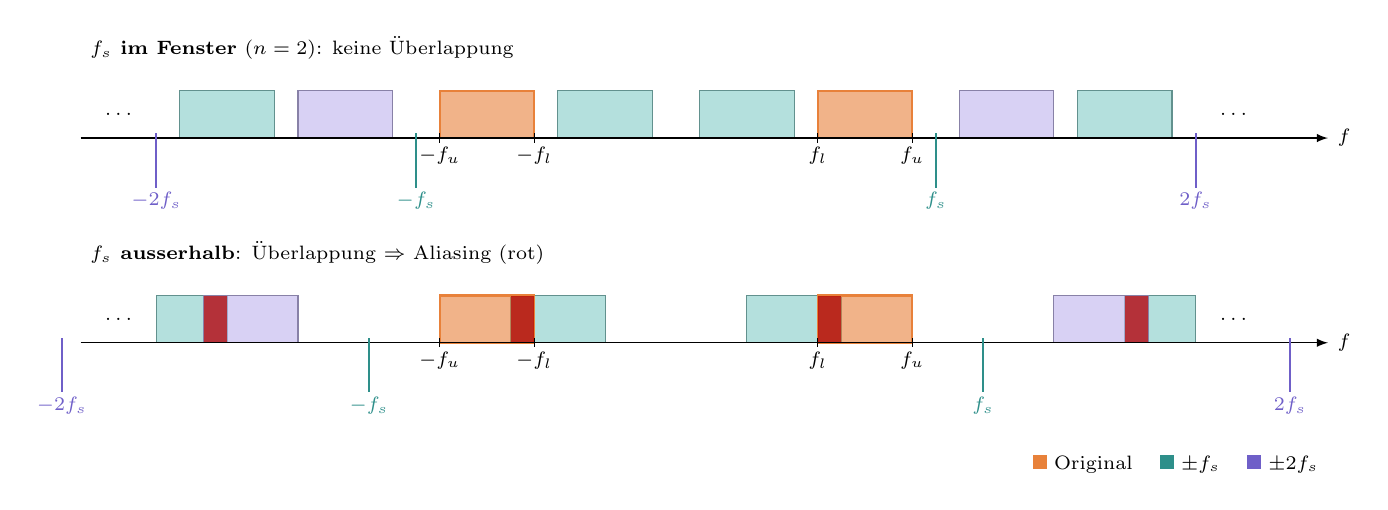
\begin{tikzpicture}[x=0.6cm,y=0.6cm,lab/.style={font=\scriptsize}]
\definecolor{org}{HTML}{E8813A}
\definecolor{kA}{HTML}{8CCFCB}\definecolor{kAd}{HTML}{2E8F8A}
\definecolor{kB}{HTML}{C3B8EE}\definecolor{kBd}{HTML}{6F5FC8}
\def\kopie#1#2#3{\fill[#3,fill opacity=0.65,draw=#3!70!black,thin] (#1,0) rectangle (#2,1);}
\def\orig#1#2{\fill[org,fill opacity=0.6,draw=org,thick] (#1,0) rectangle (#2,1);}
\def\ueber#1#2{\fill[red!70!black,fill opacity=0.75] (#1,0) rectangle (#2,1);}
\def\achse{\draw[-latex] (-12.6,0) -- (13.8,0) node[lab,right] {$f$};
  \foreach \x/\t in {-5/-f_u,-3/-f_l,3/f_l,5/f_u} \draw (\x,0.1) -- (\x,-0.1) node[lab,below,yshift=2pt] {$\t$};
  \node[lab] at (-11.8,0.5) {$\ldots$}; \node[lab] at (11.8,0.5) {$\ldots$};}
\def\ftick#1#2#3{\draw[#2,thick] (#1,0.1) -- (#1,-1.05) node[lab,below,text=#2,yshift=2pt] {$#3$};}
% Zeile 1: f_s im Fenster (f_s = 5,5)
\node[lab,anchor=west] at (-12.6,1.9) {\textbf{$f_s$ im Fenster} ($n=2$): keine Überlappung};
\kopie{0.5}{2.5}{kA} \kopie{8.5}{10.5}{kA} \kopie{-2.5}{-0.5}{kA} \kopie{-10.5}{-8.5}{kA}
\kopie{6}{8}{kB} \kopie{-8}{-6}{kB}
\orig{3}{5} \orig{-5}{-3}
\achse
\ftick{5.5}{kAd}{f_s} \ftick{-5.5}{kAd}{-f_s} \ftick{11}{kBd}{2f_s} \ftick{-11}{kBd}{-2f_s}
% Zeile 2: f_s ausserhalb (f_s = 6,5)
\begin{scope}[yshift=-2.6cm]
\node[lab,anchor=west] at (-12.6,1.9) {\textbf{$f_s$ ausserhalb}: Überlappung $\Rightarrow$ Aliasing (rot)};
\kopie{1.5}{3.5}{kA} \kopie{9.5}{11}{kA} \kopie{-3.5}{-1.5}{kA} \kopie{-11}{-9.5}{kA}
\kopie{8}{10}{kB} \kopie{-10}{-8}{kB}
\orig{3}{5} \orig{-5}{-3}
\ueber{3}{3.5} \ueber{-3.5}{-3} \ueber{9.5}{10} \ueber{-10}{-9.5}
\achse
\ftick{6.5}{kAd}{f_s} \ftick{-6.5}{kAd}{-f_s} \ftick{13}{kBd}{2f_s} \ftick{-13}{kBd}{-2f_s}
\end{scope}
\node[lab,anchor=east] at (13.8,-6.9) {\textcolor{org}{\rule{5pt}{5pt}} Original \;\; \textcolor{kAd}{\rule{5pt}{5pt}} $\pm f_s$ \;\; \textcolor{kBd}{\rule{5pt}{5pt}} $\pm 2f_s$};
\end{tikzpicture}}
\end{center}
